\chapter{Conclusiones}

\section{Conclusiones Generales}
    
    Consideramos que la práctica ha sido la más sencilla de realizar, ya que el algoritmo de Greedy, si bien nos presentó una confusión en su explicación pero en su implementación conseguimos entender el algoritmo. El problema de la práctica nos dio una vista clara a las aplicaciones de diferentes algoritmos para mejorar la vida diaria. Aunque este algoritmo no presente una solución óptima adecuada, ayuda y eso es lo que importa.

\newpage
\section{Isaac Sánchez - Conclusiones}
    El algoritmo de Greedy fue de los temas que más tuve que poner atención, no conseguí entender a la primera y tuve que conseguir ayuda extra de ciertas bibliografías. Al finalizar la práctica y hacer el análisis a priori, descubrí que hay algoritmos que pueden das soluciones a problemas tan simples como saber los días que se tienen que comprar fertilizante sin requerir una complejidad tan complicada. 
    \begin{figure}[htp!]
            \centering
            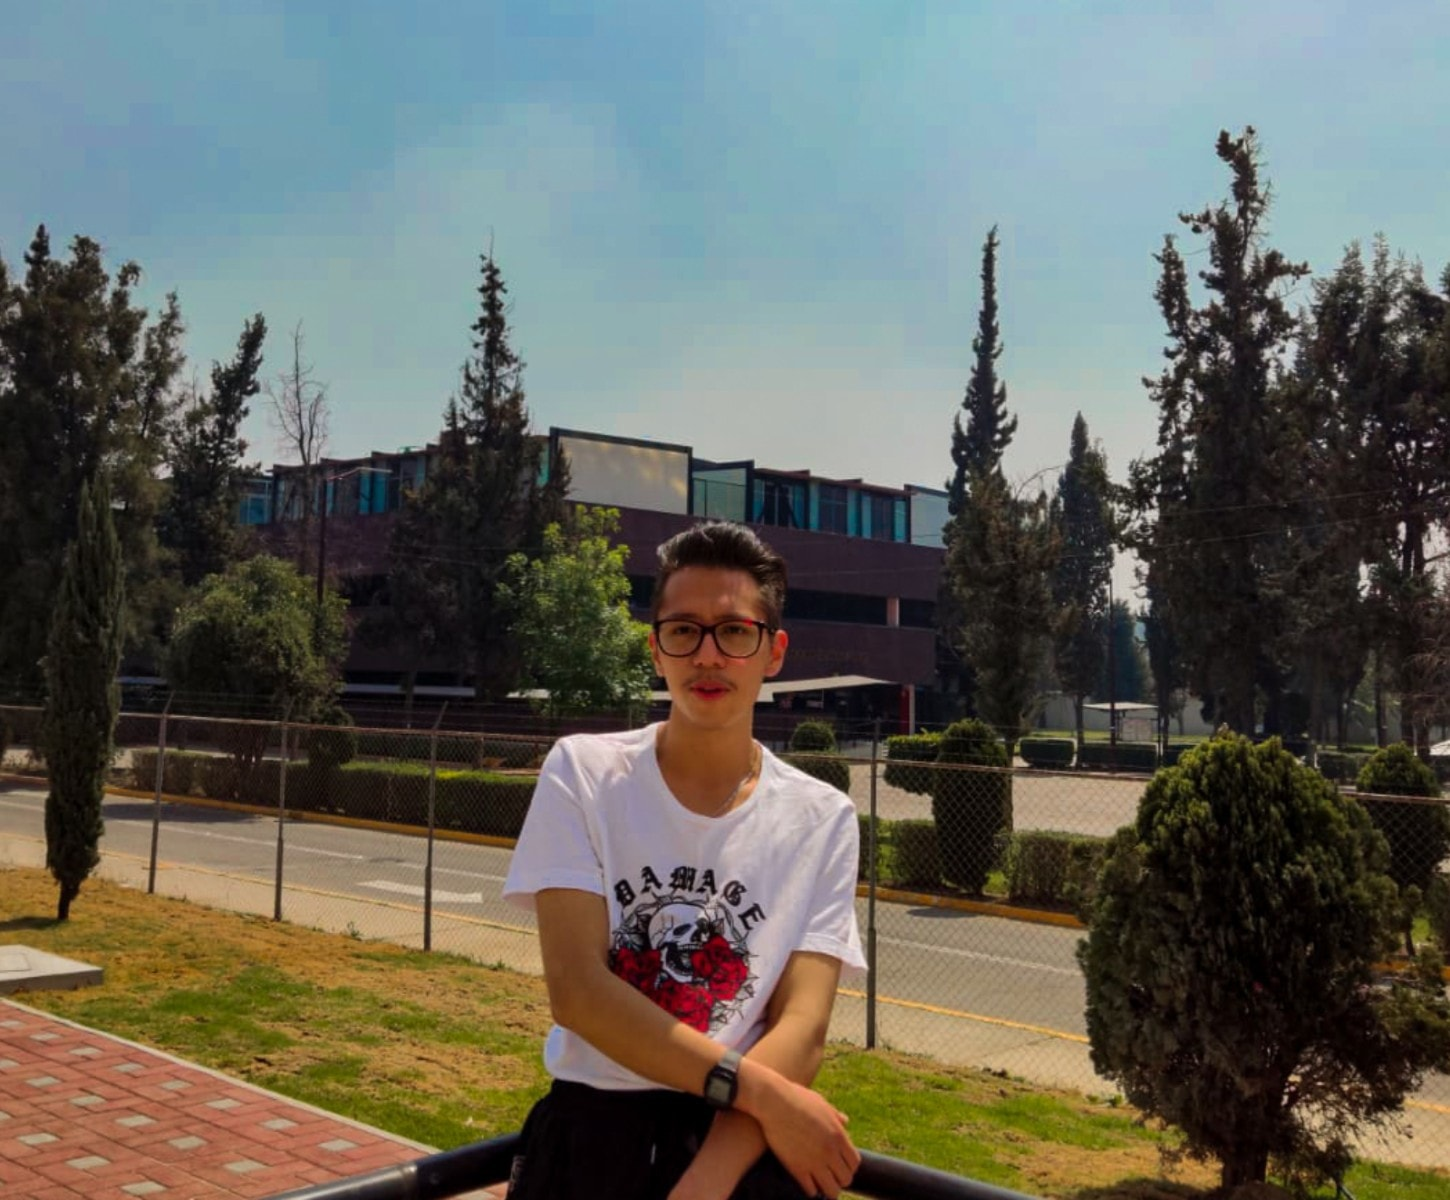
\includegraphics[width=1 \textwidth]{Images/Fotos_Alumnos/274612600_2528992867236334_6677874837890685705_n.jpg}  
            \caption{Isaac Sánchez}
            \label{fig:my_label1}
        \end{figure}
    


\newpage
\section{Axel Trevino - Conclusiones}
    La práctica fué un buen ejemplo de el algoritmo greedy, porque es un uso en la vida real que le podrías dar. Lo único malo del greedy es que no te puede ayudar si no conoces bien los días en los que abre la tienda, o si puedes comprar cuanto fertilizante como quieras; como siempre, un algoritmo no resuelve vidas, sólo las hace más fáciles.
    \begin{figure}[htp!]
            \centering
            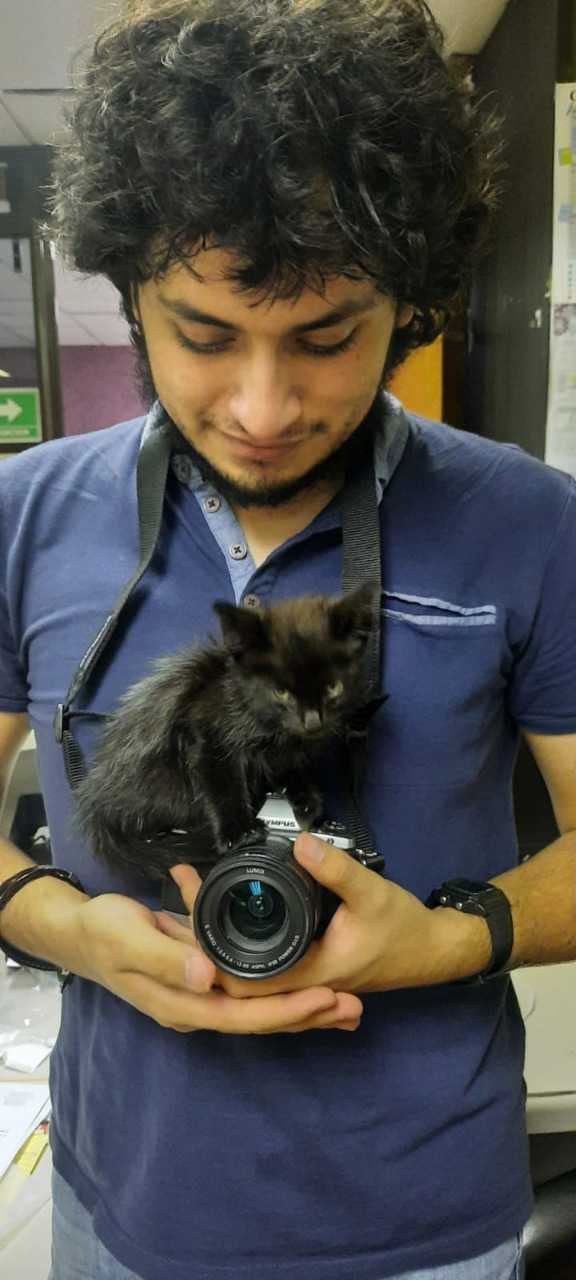
\includegraphics[width=0.4 \textwidth]{Images/Fotos_Alumnos/axel.jpg}  
            \caption{Axel Treviño}
            \label{fig:my_label2}
        \end{figure}
